\documentclass[%
 reprint,
%superscriptaddress,
%groupedaddress,
%unsortedaddress,
%runinaddress,
%frontmatterverbose, 
%preprint,
%preprintnumbers,
%nofootinbib,
%nobibnotes,
%bibnotes,
 amsmath,amssymb,
 aps,
%pra,
%prb,
%rmp,
%prstab,
%prstper,
%floatfix,
]{revtex4-2}

\usepackage{graphicx}% Include figure files
\usepackage{dcolumn}% Align table columns on decimal point
\usepackage{bm}% bold math
\usepackage{hyperref}% add hypertext capabilities
\hypersetup{
    colorlinks=true,
    linkcolor=red,
    citecolor=blue,      
    urlcolor=magenta,
}
%\usepackage[mathlines]{lineno}% Enable numbering of text and display math
%\linenumbers\relax % Commence numbering lines

%\usepackage[showframe,%Uncomment any one of the following lines to test 
%%scale=0.7, marginratio={1:1, 2:3}, ignoreall,% default settings
%%text={7in,10in},centering,
%%margin=1.5in,
%%total={6.5in,8.75in}, top=1.2in, left=0.9in, includefoot,
%%height=10in,a5paper,hmargin={3cm,0.8in},
%]{geometry}

\begin{document}

\preprint{APS/123-QED}

\title{Using a Recursive Neural Network to Generate Tweets}% Force line breaks with \\

\author{Victoria Kovalchuk}
\author{Kaitlin Salyer}%
\affiliation{%
 Boston University Department of Physics\\
 590 Commonwealth Ave.\\
 Boston, MA 02215
}%

\date{17 December 2019}

\begin{abstract}
The goal of this project is to build a Twitter bot. Using tweepy, the Python package for extracting and utilizing information from Twitter (Twitter Application Program Interface), we extract the most recent tweets from a username of choice or with a specific hashtag. These tweets will be included in a text file used for training a recursive neural network designed using another Python package, textgenrnn. Textgenrnn is a package which allows the user to design the architecture of an RNN and train the model with any desired dataset. This trained model can then generate its own tweets and tweet them out from the Jupyter notebook if desired. Using these packages, we acheive the goal of building a Twitter bot, and train the model on three datasets: Ariana Grande tweets, Chrissy Teigen tweets, and Greta Thunberg tweets.
\end{abstract}

%\keywords{Suggested keywords}%Use showkeys class option if keyword
                              %display desired
\maketitle

%\tableofcontents

\section{Introduction}

The goal of this project was to utilize a recursive neural network (RNN) to generate tweets in the style or theme specified by the operator. In this report, we show examples of models trained to tweet like Chrissy Teigen, Ariana Grande, and Greta Thunberg.

In order to understand the content of this report, it is important to understand how the textgenrnn Python package works, as this is the basis of what was used to accomplish the goal. A flowchart describing how the default RNN is constructed in the package is outlined in Figure \ref{fig:textgenrnn}.

It begins with the input layer, which takes an input of 40 characters maximum and feeds it to an embedding layer which converts each character to a vector. It does this by assigning each character a 1-hot vector of 100 dimensions. This information is then passed to the next layer: a Long Short-Term Memory (LSTM) layer. \cite{textgenrnnDoc}

An LSTM is an artificial RNN architecture: this means that it differs from basic feed-forward neural networks because it has feedback connections. The benefit of RNNs is that they can keep track of long-term dependencies in the input information. The weakness associated with this is that, during back-propagation, the gradients have a tendency to either vanish or blow up to infinite values. LSTMs solve the vanishing gradient problem by allowing gradients to flow unchanged. This, however, does not solve the infinite gradient problem, so that needs to be considered in the process of using RNNs. The default RNN structure of the textgenrnn package has two LSTM layers, each with 128 cells (the unit of memory in LSTMs).\cite{LSTMpaper}

The output of the first LSTM is fed into the second one, but the output of both of these LSTMs and the previous embedding layer is fed to into an attention layer for purposes of weighting the most important temporal features and then averaging them. The fact that all three of the previous layers are fed separately into this one allows for easy back-propagation for the prevention of vanishing gradients. The output is then mapped to probabilities for up to 394 characters that they are the next character in the sequence. These probabilities are for upper and lowercase letters, punctuation, and emojis. All of these numerical features can be adjusted in the design of the model; however, for the purposes of this project, we kept them the same. \cite{textgenrnnDoc}

One important note about this attention layer is that, because it takes as input the output of the previous three layers, it is better to design a network that is deeper, rather than wider. By this, we mean that a 4-layer, 128-cell network will likely perform better than a 1-layer 512-cell network. The exception to this is in the case of a very large amount of input text. Because we are working with tweets, which are limited to 280 characters, we abided by the rule that deeper is better than wider. \cite{maxWoolfBlog}

\begin{figure}[h]
    \centering
    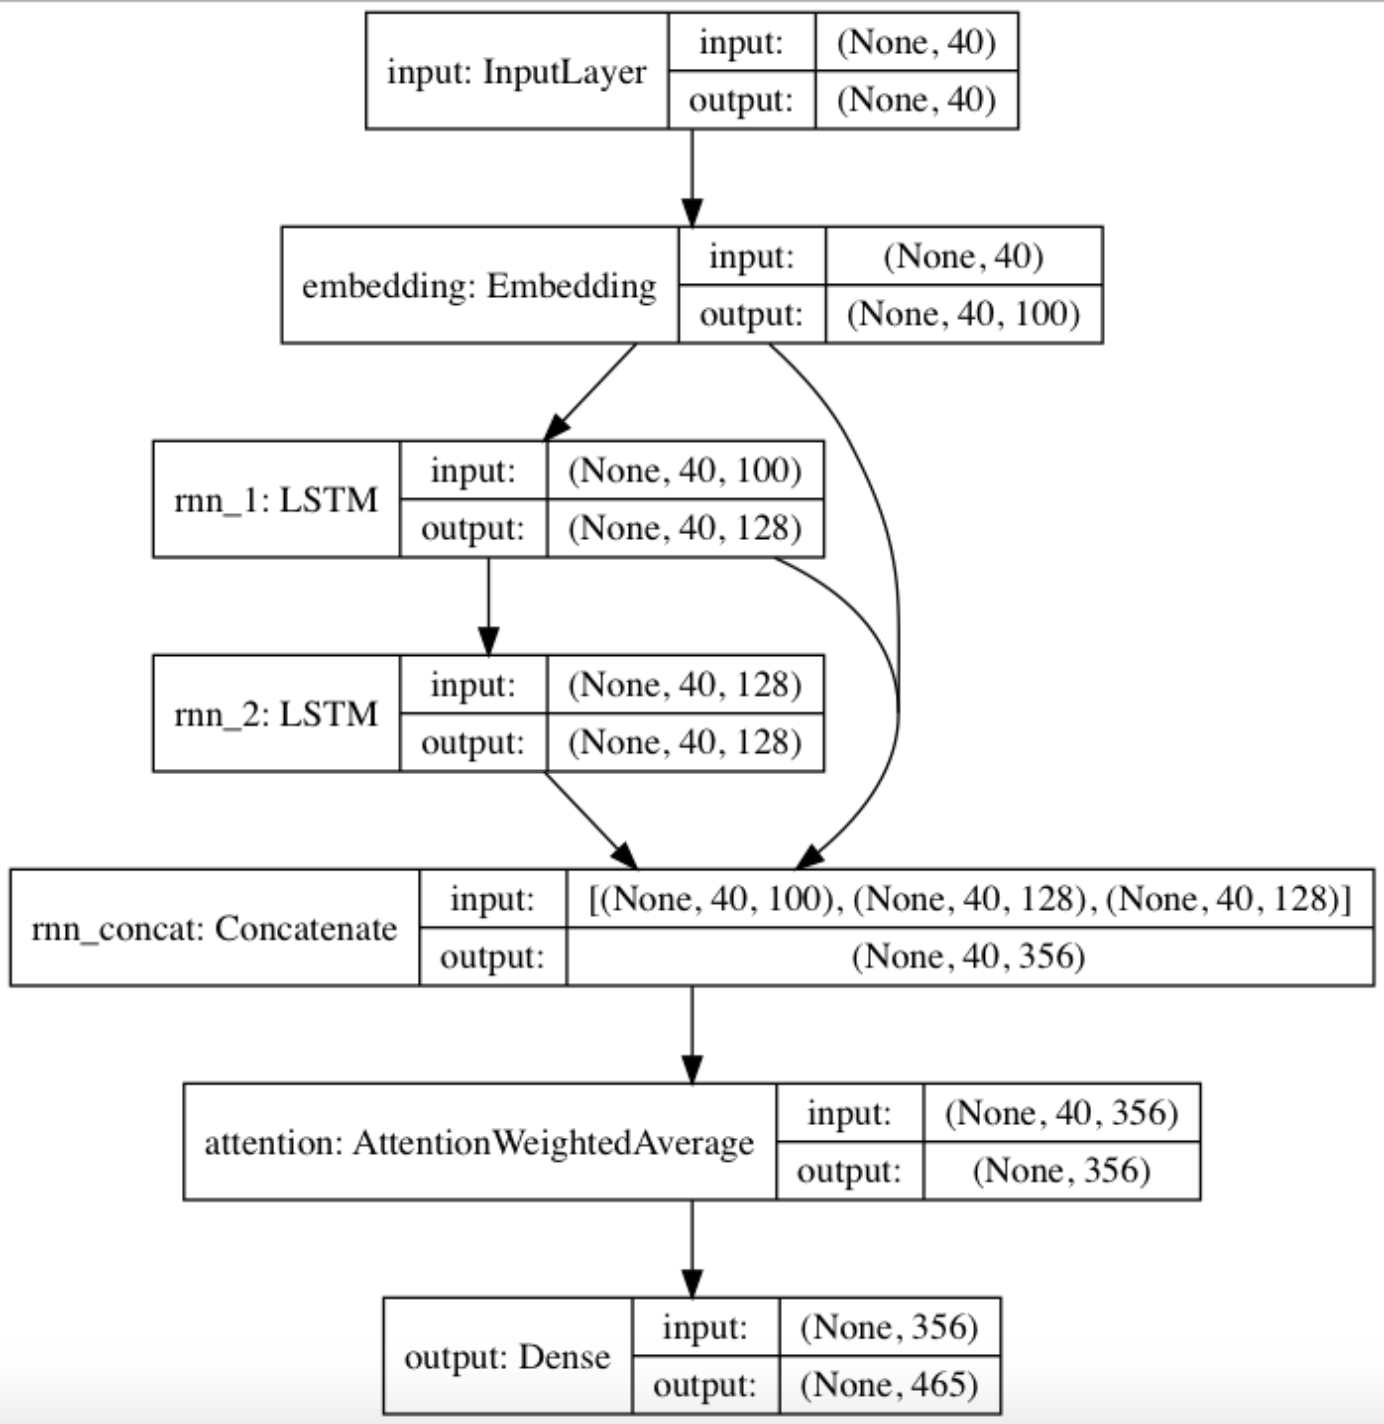
\includegraphics[scale=0.35]{textgenrnnPackageFlowchart.png}
    \caption{Flowchart visualizing the structure of the RNN designed by the textgenrnn Python package.}
    \label{fig:textgenrnn}
\end{figure}

\section{Methods and Materials}

Materials necessary for this project are as follows:
\begin{itemize}
    \item tweepy: Twitter API Python package
    \item textgenrnn: Text-generating Recursive Neural Network package for Python which also utilizes the following packages:
    \begin{itemize}
        \item numpy
        \item tensorflow
    \end{itemize}
\end{itemize}
These were applied in a Jupyter notebook, using Anaconda software.

\section{Procedure}

The procedure can be broken down into two main steps: making a dataset and training the RNN. We will discuss each of these steps in detail.

\subsection{Making a Training Set}
It is necessary to create a training dataset before anything else. This can be done by writing a code for extracting and saving to a text file tweets from a specific username or from a specific hashtag. Using tweepy, there are a number of useful functions that can be called and makes this process easier. 

First, you feed the security and authorization information to the system so that it can read Twitter accounts and feeds. It is possible to filter based off of date, content, sentiment expressed, among other things, but for the purposes of this project, we decided to just take all of the most recent tweets. Twitter allows for a maximum of 3200 tweets to be extracted via this method, so we were limited by that number. The functions operate by going into the feed and selecting a collection of 100 tweets at a time, making sure they meet the filters applied, and then appending the tweet content to the output text file. It is then important to make sure that the next time that it pulls 100 tweets, that those are not the same tweets from the last iteration. This is applied as an if/else statement in the code on our Github pages: \href{https://github.com/vvk3da/PY895ML/tree/master/FinalProject}{Victoria's} and \href{https://github.com/ksalyer/py895/tree/master/FinalProject}{Kaitlin's}.

\subsection{Training the Model}

The most important step in this procedure is the designing of the architecture of the model and training it. Using the functions defined in the textgenrnn package, we can define the dimensions of our network (that is, how many layers deep and how many cells wide the network is), how many training epochs we go through, the size of the training batches, and many more features. These are the nobs that we are able to turn to tune our model to the best possible outcome. There is a ``train\_from\_file" function that we call to train the model with the text file we made in the previous step. During the training process, the function returns to the command line the estimated loss and generated tweets at various ``temperatures" at the end of each epoch. These temperatures are various levels of creativity \cite{maxWoolfBlog}, so to speak. A temperature of 0.2 allows for more suboptimal prediction, whereas a temperature of 1 gives a very well-trained model. An example of this can be seen in Figures \ref{fig:ChrissyTeigen}, \ref{fig:ArianaGrande}, and \ref{fig:GretaThunberg}. These printouts give the user the opportunity to see how much the algorithm improves with each epoch and if any tweaks should be made to the architecture. When the training is finished, the function writes the configuration, vocabulary, and weights to separate output files. With these three files, you can generate a tweet from the already trained model. 

\begin{figure}[h]
    \centering
    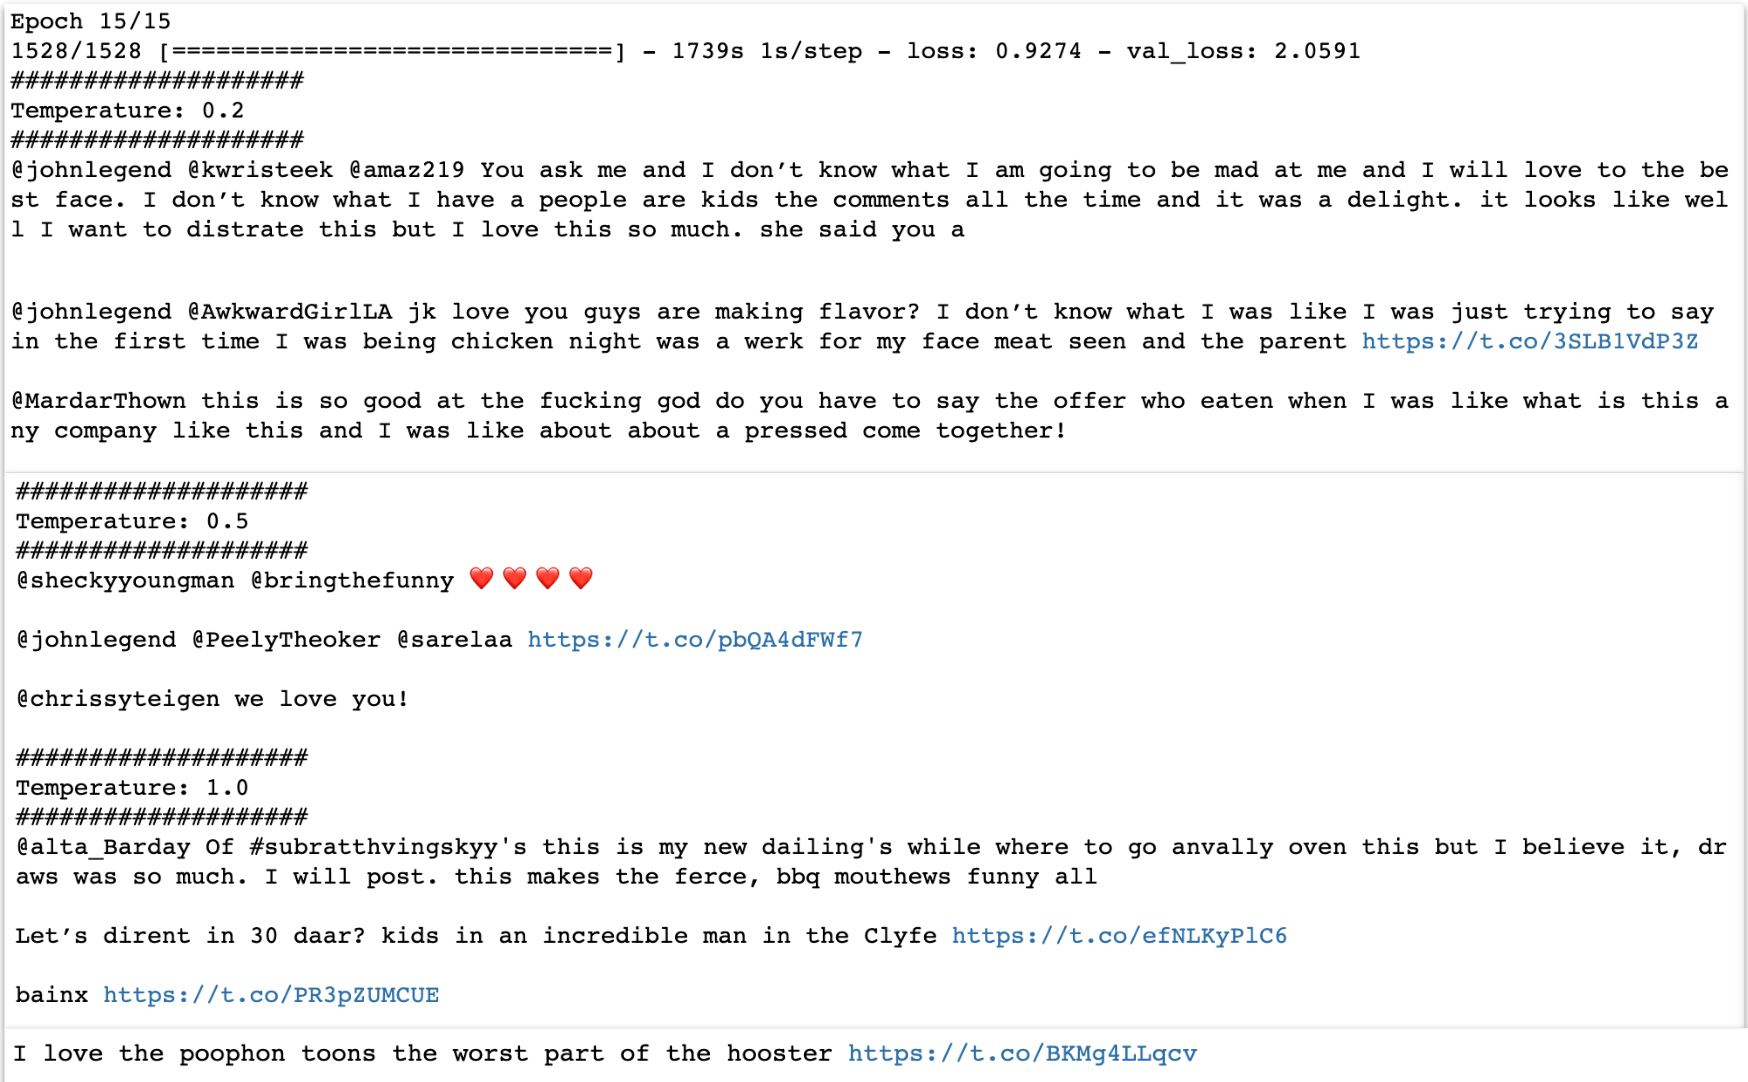
\includegraphics[scale=0.28]{ChrissyTeigenResults.png}
    \caption{Printout from training the model with Chrissy Teigen tweets. This model was trained with 15 epochs, 6 layers and 128-cell LSTMs.}
    \label{fig:ChrissyTeigen}
\end{figure}

\begin{figure}[h]
    \centering
    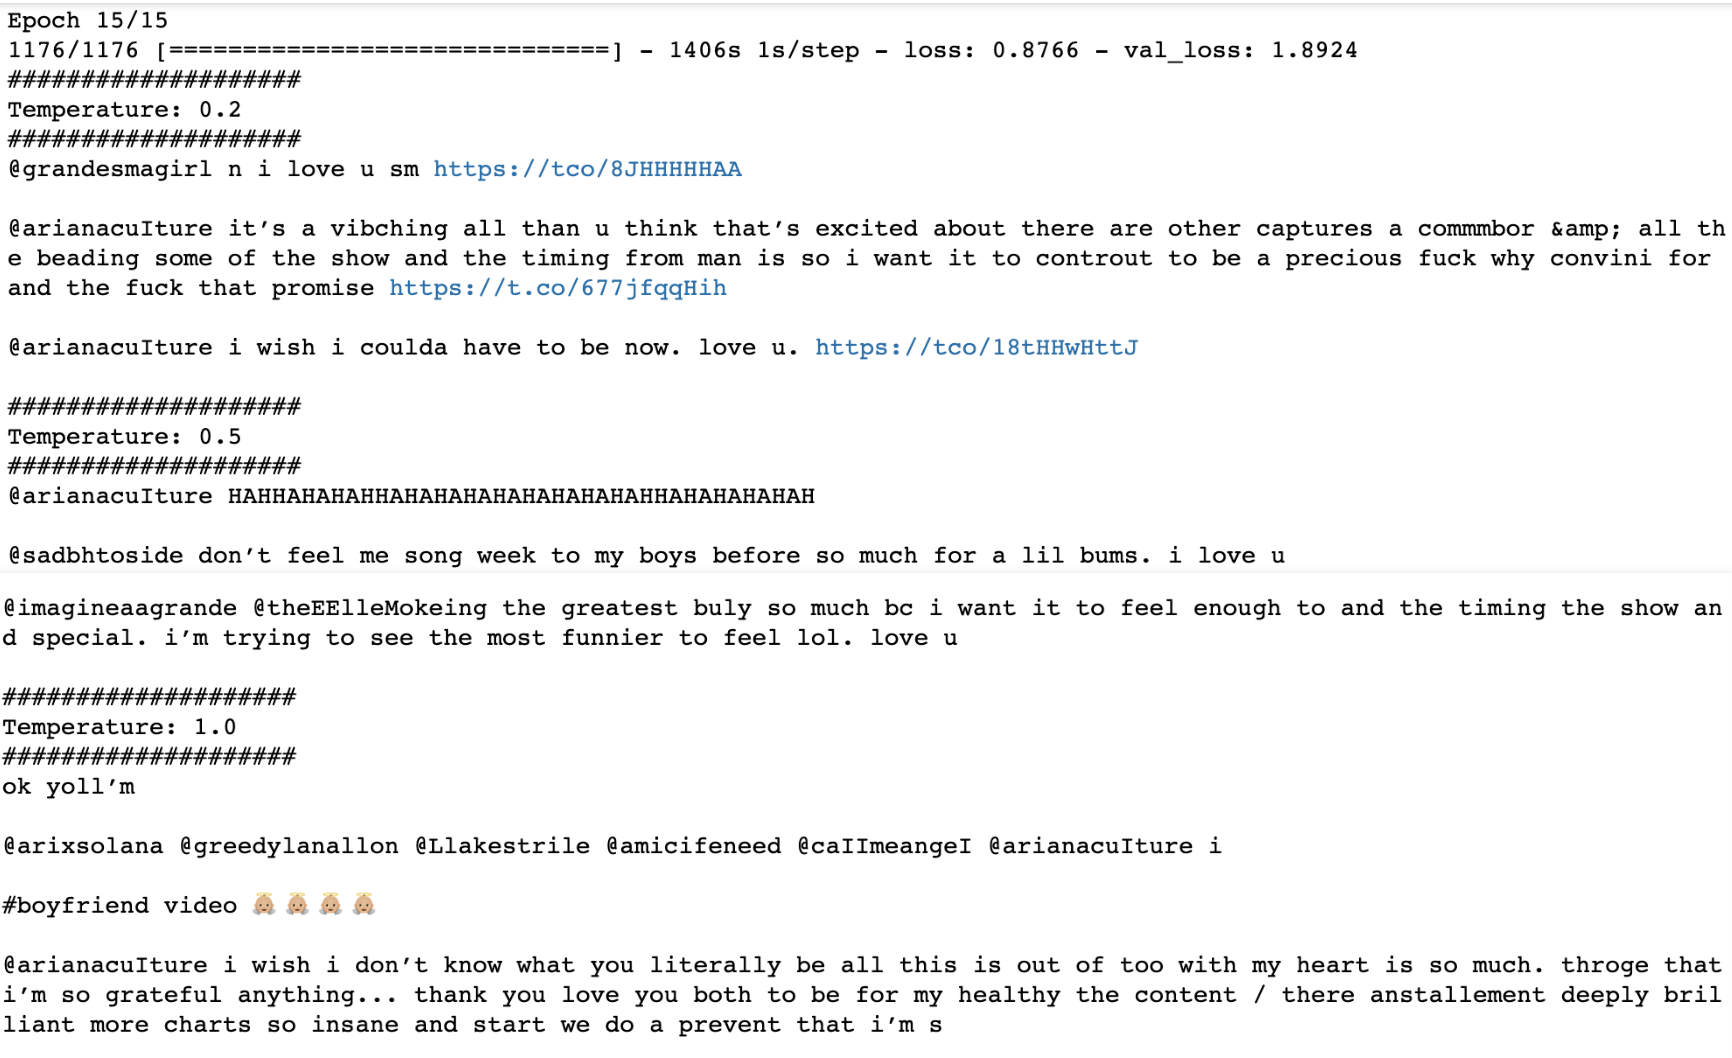
\includegraphics[scale=0.28]{ArianaGrandeResults.png}
    \caption{Printout from training the model with Ariana Grande tweets. This model was trained with 15 epochs, 6 layers and 128-cell LSTMs.}
    \label{fig:ArianaGrande}
\end{figure}

\section{Results}

The results of the final epoch of each training is visible in Figures \ref{fig:ChrissyTeigen}, \ref{fig:ArianaGrande}, and \ref{fig:GretaThunberg}. The model worked best in all three datasets with a slightly forgiving temperature of 0.5, and the results were most coherent with the relatively simple dataset of Ariana Grande tweets. The goal of creating a tweet generator was accomplished.

\begin{figure}
    \centering
    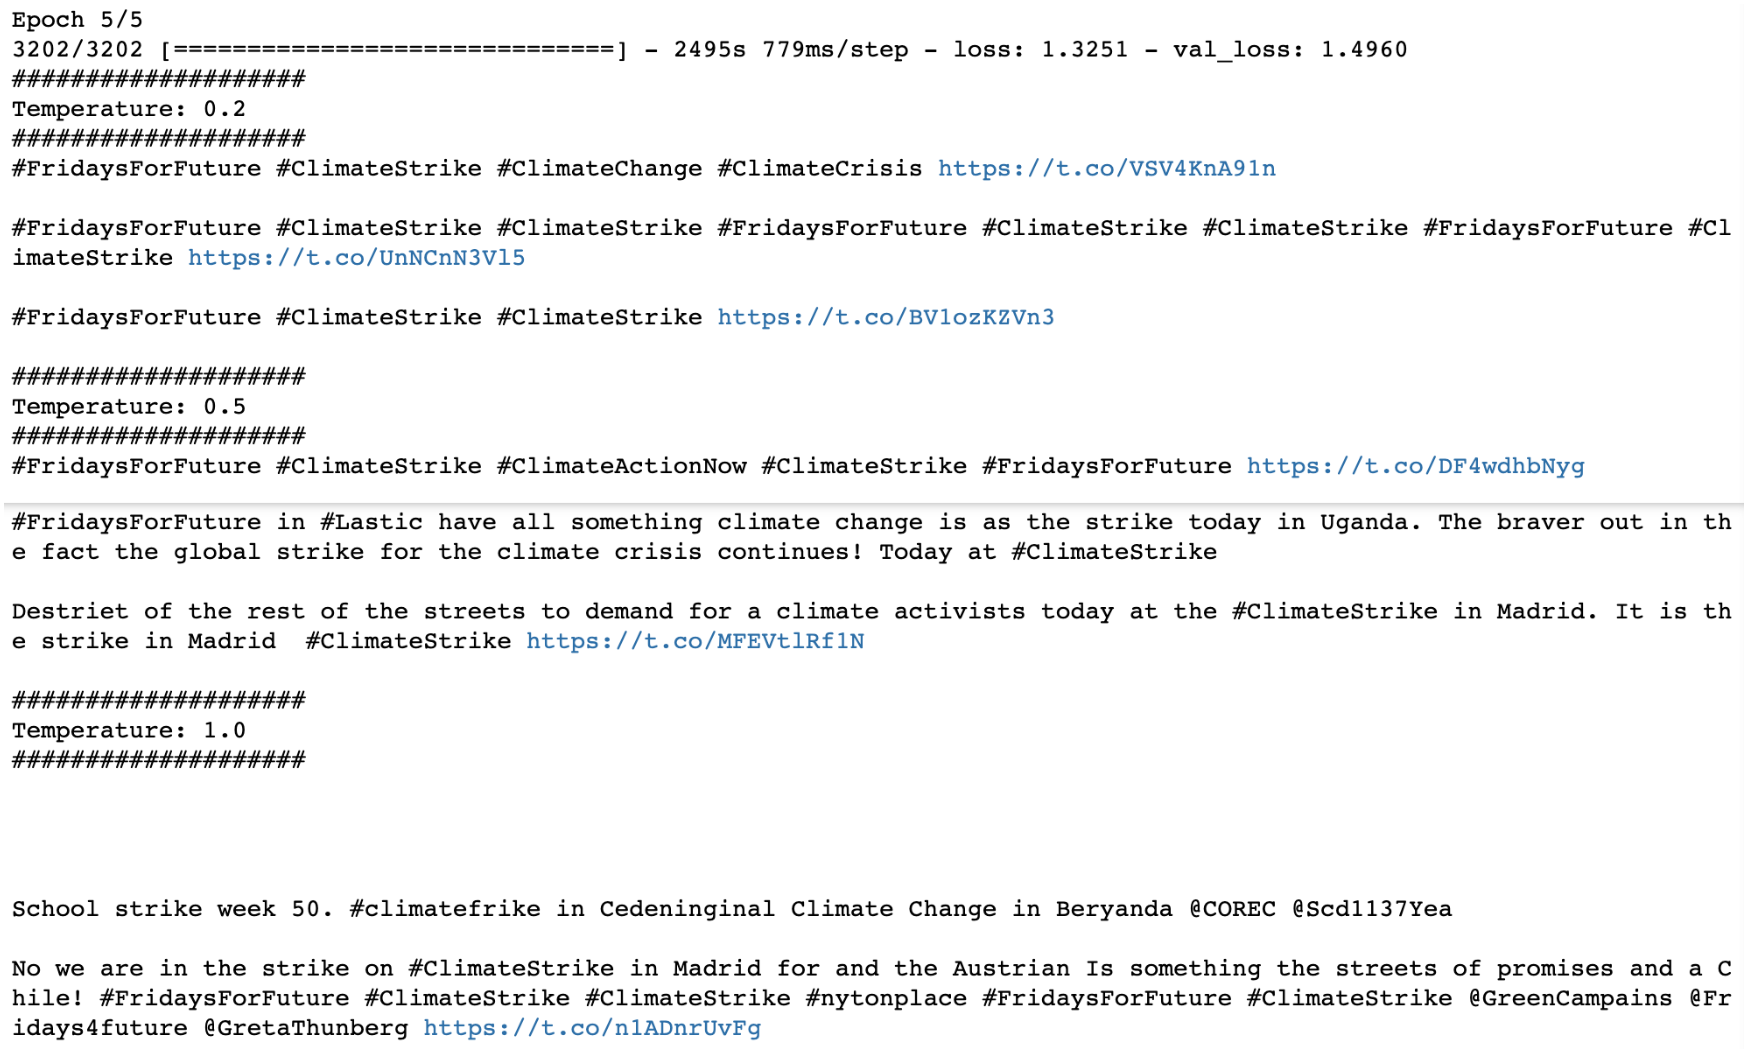
\includegraphics[scale=0.28]{GretaThunbergResults.png}
    \caption{Printout from training the model with Greta Thunberg tweets. This model was trained with 5 epochs, 4 layers and 128-cell LSTMs.}
    \label{fig:GretaThunberg}
\end{figure}

\section{Discussion}

We intended to use the same architecture for training all three models, but the Anaconda kernel kept failing during the training on Greta Thunberg data. Training on her tweets took a significantly longer time per epoch than the other datasets, so we trained a simpler model with her data. Furthermore, the three datasets were unique in their own ways. Ariana Grande's tweets tend to follow a very similar form. Usually they are short and she repeats a lot of the same phrases. There is a lot more variance in how both Chrissy Teigen and Greta Thunberg tweet, but Greta's account has the added training difficulty of having more than just English tweets. She has tweets in her native Swedish, for example, which would also make it into the training set. Because the datasets are more complicated, they would require a more complex model to achieve the same level of coherence as the Ariana Grande model. This might be best achieved with more layers, the application of dropout, or it might be worth including more input characters at the beginning, rather than the default 40. Perhaps the extended training time we encountered for Greta Thunberg's dataset was caused by the relative complexity of the data. Testing these theories would be valuable next steps in this investigation.

By completing this project, we have seen that creating a twitter-bot is a lot easier than it seems. Using the textgenrnn package simplifies the writing process significantly: the code to train three models is less than 100 lines. It costs mostly just computing time and resources, but this would be dramatically reduced on a GPU as opposed to our local computers. The author of the package said the speed per training epoch on a GPU is fourteen times faster than a CPU \cite{maxWoolfBlog}. 

\bibliography{ML_FinalPaper.bib}% Produces the bibliography via BibTeX.

\end{document}
%
% ****** End of file apssamp.tex ******
